% ============================================================
% Chapter: Changes in the geometry of hippocampal representations across brain states
% Yang, Sun, Buzsáki. NeurReps / NeurIPS Workshop 2023.
% ============================================================

\blfootnote{This chapter is adapted from: Wannan Yang, Chen Sun, and György Buzsáki.
``Changes in the geometry of hippocampal representations across brain states.''
\textit{NeurReps: Symmetry and Geometry in Neural Representations Workshop, NeurIPS} (2023).
Wannan Yang is first author.}

\section*{Abstract}

The hippocampus (HPC) is a key structure of the brain's capacity to learn and generalize. One pervasive phenomenon in the brain, but missing in AI, is the presence of different gross brain states. It is known that these different brain states give rise to diverse modes of information processing that are imperative for hippocampus to learn and function, but the mechanisms by which they do so remain unknown. To study this, we harnessed the power of recently developed dimensionality reduction techniques to shed insight on how HPC representations change across brain states. We compared the geometry of HPC neuronal representations when rodents learn to generalize across different environments, and showed that HPC representation could support both pattern separation and generalization. Next, we compared HPC activity during different stages of sleep. Consistent with the literature, we found a robust recapitulation of the previous awake experience during non rapid eye movement sleep (NREM). But interestingly, such geometric correspondence to previous awake experience was not observed during rapid eye movement sleep (REM), suggesting a very different mode of information processing. This is the first known report of UMAP analysis on hippocampal neuronal data during REM sleep. We propose that characterizing and contrasting the geometry of hippocampal representations during different brain states can help understand the brain's mechanisms for learning, and in the future, can even help design next generation of AI that learn and generalize better.

\bigskip
\noindent\textbf{Keywords:} UMAP, memory, hippocampus, REM sleep, learning, generalization

\section{Introduction}

Memory storage in the brain goes through a two-stage process \citep{marr1971simple, buzsaki1989two}. First, behavioral episodes are rapidly encoded by the key structure called the hippocampus during awake behavior \citep{whittington2020tolman}. The fast-learning mechanisms of the hippocampus ensures quick and efficient encoding of memories, even down to single-trials \citep{tulving2002episodic}. However, these representations are vulnerable to interference by newly encoded information. Therefore, new information needs to be gradually integrated to a different learning system during other brain states (for example, REM and NREM sleep). However, the learning mechanisms themselves during those brain states are unknown. In AI, incorporating a sleep-like offline learning stage has started to demonstrate increasingly promising results to support robust learning and generalization \citep{hafner2022mastering, ellis2020dreamcoder, mnih2013playing, hinton1995wakesleep, sun2022contrastive}, but truly harnessing mechanisms of learning through different states akin to those seen in the brain is an area of research in its infancy.

In this paper, we study how hippocampal neuronal representations topologically change across brain states (awake task learning, different stages of sleep, novel learning). Our key contributions are as follows:
\begin{itemize}
    \item HPC representations in the awake state can support both pattern separation and generalization.
    \item HPC representation during REM sleep implies a different form of memory processing beyond faithful reactivation of the recent episodic experience, unlike during NREM sleep.
\end{itemize}

\section{Methods}

To date, most efforts to characterize neuronal representation between brain states are supervised methods, which are based on template-matching principles to compare patterns between behavioral states \citep{chaudhuri2019intrinsic, rubin2019revealing}. Such supervised approaches are limited because they use one of the brain states (usually during awake learning) to impose an \textit{a priori} template derived from the external world, in order to analyze another brain state (e.g. sleep), resulting in the neglect of important features intrinsic to sleep. Here, we apply recently developed unsupervised approaches \citep{mcinnes2020umap, bernardi2020geometry} to study hippocampal representations, uncovering their intrinsic neuronal activity structure, without needing to match to a template imposed by the external world. First, we applied multidimensional scaling (MDS) \citep{bernardi2020geometry} to discover shared features in the neuronal representations during generalization across sessions. Second, we applied Uniform Manifold Approximation and Projection (UMAP) for dimension reduction \citep{mcinnes2020umap} to visualize the intrinsic representation of the brain during different brain states, and compare manifold representations across brain states (Figure~\ref{fig:nreps_appA1}, Figure~\ref{fig:nreps_appB1}, Figure~\ref{fig:nreps_appC1}).

\section{The Geometry of Neural Representation During Novel Maze Learning}

The ability to separate different experiences is a critical feature of episodic memory and has long been hypothesized to require the hippocampus \citep{yassa2011pattern}. But the capacity to pattern separate between situations may impair the capacity to generalize across those situations, and there is still no general consensus to what extent hippocampal pattern separation is not at the expense of forming invariant and generalizable representation.

To explore this question, we used MDS to characterize the hippocampal representations when rodents apply the rule learned in a familiar maze and generalized it to a novel environment (Figure~\ref{fig:nreps_fig1}A). Interestingly, here we show that the HPC representation can simultaneously support both pattern separation as well as generalization through `analogy-like' representation (Figure~\ref{fig:nreps_fig1}B) \citep{bernardi2020geometry}. In this form of representation, activity of different experiences is pattern separated but are also organized such that the vectors of analogous elements of the different experiences are parallel (for example, the vector connecting the left and right reward in familiar maze is parallel to the left-right reward vector in the novel maze). In a way, this hippocampal capacity to analogize between experiences, is somewhat akin to the analogy-like word embeddings generated by word2vec from natural language processing, as exemplified by the well-known ``woman is to queen as man is to king'' \citep{mikolov2013efficient}.

\begin{figure}[htbp]
    \centering
    \includegraphics[width=0.85\textwidth]{figures/ch_nreps2023/fig1.png}
    \caption[Novel maze geometry: pattern separation and analogy-like generalization]{%
    \textbf{Hippocampal representations support both pattern separation and analogy-like generalization.}
    (A) Figure-8 maze task, where mice alternated between left and right arms for water reward (blue droplets). The animal's trajectory along maze corridors is color-coded by linearized position. Left, familiar maze where the animal was trained for one week. Right, novel maze in a novel context where the mouse was introduced for the first time.
    (B) MDS plot showing the dimensionality-reduced firing rates for familiar (red) and novel (green) mazes. The parallel alignment of analogous position vectors across environments reflects simultaneous pattern separation and generalization.}
    \label{fig:nreps_fig1}
\end{figure}

\section{The Geometry of Neural Representation During Different Sleep States}

Sleep in mammals consists of two core stages: NREM and REM sleep, which alternate in a cyclic manner \citep{rasch2013sleep, stickgold2005sleep, stickgold2013parsing}. Reactivation of memory (replay) during NREM sleep and its role in memory have been extensively studied \citep{buzsaki2015hippocampal, axmacher2008ripples, fernandezruiz2019long, foster2017replay, jadhav2012awake, rudoy2009strengthening}. Much less is known about the representations during REM sleep.

Using UMAP, we first visualized the neural representation when rodents learned in a figure-8 maze (Figure~\ref{fig:nreps_fig2}A,B). Next, we visualized the geometric structure of representations during NREM sleep. Interestingly, we uncovered a substructure that resembled the geometry of the maze (red dashed line) during NREM sleep. To test if this substructure was actually related to activity during maze exploration, we projected the population activity during maze learning to the space defined by the NREM sleep. We found that indeed, that sub-structure during NREM sleep covered the manifold of activity seen during the maze running with high precision (Figure~\ref{fig:nreps_fig2}C,D). Consistent with known literature \citep{buzsaki2015hippocampal, axmacher2008ripples, fernandezruiz2019long, foster2017replay, jadhav2012awake, rudoy2009strengthening}, this directly demonstrates that NREM sleep faithfully reactivated activity from previous behavior and likely helped to consolidate the recent episodic memory. Surprisingly, we were able to demonstrate this using an unsupervised technique where the maze-like substructure in the NREM manifold naturally emerged without being forced to match with any pre-defined template, and was therefore a much stronger result comparing to previous template-matching methods.

\begin{figure}[htbp]
    \centering
    
\includegraphics[width=\textwidth]{figures/ch_nreps2023/fig2.png}
    \caption[UMAP geometry of hippocampal representations across brain states]{%
    \textbf{UMAP reveals distinct hippocampal geometry during NREM and REM sleep.}
    (A) Figure-8 maze task. The animal's trajectory is color-coded by linearized position.
    (B) UMAP embedding of population activity during maze running. Manifold is colored by linearized position.
    (C) UMAP manifold of NREM sleep.
    (D) Projecting maze data onto the manifold of NREM sleep.
    (E) and (F) are similar to (C) and (D) but for REM sleep. The absence of maze-like structure during REM suggests a qualitatively different mode of information processing.}
    \label{fig:nreps_fig2}
\end{figure}

In contrast, we did not observe a maze-like structure during REM sleep (Figure~\ref{fig:nreps_fig2}E,F), suggesting a different role other than faithful reactivation of the recent episodic experience. Compared to NREM sleep, REM sleep events have a longer distance to manifold and trajectory length (Figure~\ref{fig:nreps_fig3}A,B). The two quantities were also used to determine if a candidate sleep event is a significant replay event by comparing it to shuffle (Figure~\ref{fig:nreps_appA1}). The fraction of significant REM replay events is not statistically different from that of shuffle events (Figure~\ref{fig:nreps_fig3}C, Figure~\ref{fig:nreps_appC1}).

\begin{figure}[htbp]
    \centering
    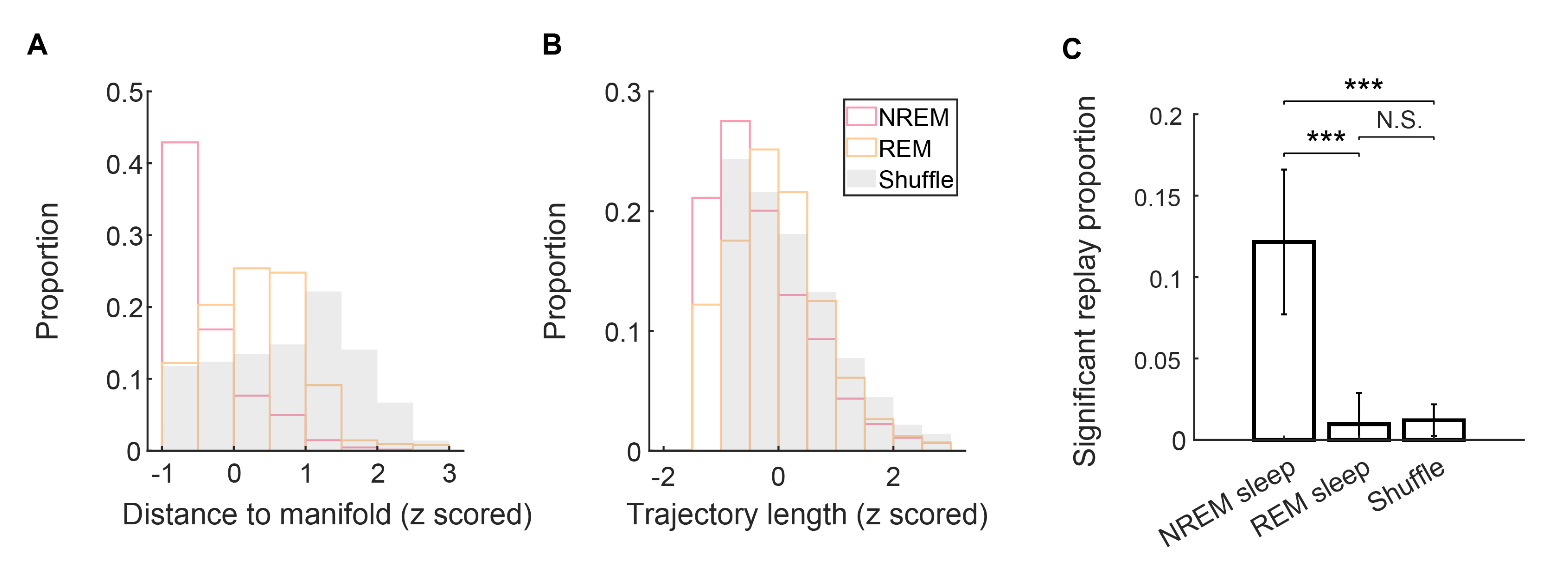
\includegraphics[width=\textwidth]{figures/ch_nreps2023/fig3.png}
    \caption[Quantification of replay across brain states]{%
    \textbf{Replay statistics differ markedly between NREM and REM sleep.}
    (A) Distribution of distance to maze manifold for replay events across different brain states.
    (B) Distribution of trajectory length.
    (C) Proportion of significant replay events across different brain states. The fraction of significant REM replay events is not statistically different from that of shuffle, in contrast to NREM sleep.}
    \label{fig:nreps_fig3}
\end{figure}

Our results suggest that the interleaving NREM and REM sleep epochs play different roles during system consolidation. Our results for REM sleep suggest that we might need to update our understanding for the role of REM sleep. In particular, previous studies \citep{zielinski2021hippocampal, louie2001temporally} claimed that replay of maze events seems to present during REM sleep, suggesting that REM sleep plays a similar role as NREM sleep for faithfully reconstructing and replaying the recent episodic experience. However, both of those papers used supervised or template-matching methods. In light of our new results, it is possible that the role of REM sleep is to facilitate the abstraction of general rules from the combinations of many different past experiences \citep{lewis2018memory}, and might therefore not possess faithful reactivation of the most recent experience during this brain state, at all. To our knowledge, this is the first reported characterization of hippocampal population activity during REM sleep using UMAP analysis (or unsupervised dimensionality reduction method in general).

\section{Discussion and Future Directions}

Our result showing hippocampal representations during active rodent behavior generalizing to a new maze provides novel insight into how hippocampal representation can support both pattern separation of episodic experience in different contexts as well as harbor generalizable representation that can support rapid generalization. By harnessing a linear dimensionality reduction (MDS) we are able to bridge divergent findings showing that HPC representations support pattern separation \citep{yassa2011pattern, samborska2022complementary, tang2023geometric} and other studies showing HPC representations can also support generalization \citep{quiroga2005invariant, sun2020}. However, this is a preliminary result, and further experiments (for example, in a diverse set of tasks) are needed.

Secondly, our results point to critical differences in information processing by the hippocampus during REM vs. NREM sleep. To our knowledge, ours is the first study to characterize hippocampal neuronal activity during REM sleep by UMAP analysis, giving us the capacity to see beyond previous studies on REM sleep that used single neuron analysis or template-matching based decoding analysis. This preliminary result presents an insightful snapshot into hippocampal activity during learning and memory. Future work should aim to characterize hippocampal representational changes over the entire timecourse of learning. This study is a first step to uncover the mysterious role of different brain states (especially during sleep) for learning about the world.

\subsection*{Acknowledgments}

We thank the members of the Buzsáki lab for helpful discussions, and Chen Sun for collaboration on the figure-8 maze dataset.
